
\documentclass[10pt,a4paper]{article}
\usepackage{f1000_styles}

%% Default: numerical citations
% \usepackage[numbers]{natbib}

%% Uncomment this lines for superscript citations instead
% \usepackage[super]{natbib}

%% Uncomment these lines for author-year citations instead
% \usepackage[round]{natbib}
% \let\cite\citep

%% lines required to use a CSL style for references
\newlength{\cslhangindent}
\setlength{\cslhangindent}{1.5em}
\newlength{\csllabelwidth}
\setlength{\csllabelwidth}{3em}
\newlength{\cslentryspacingunit} % times entry-spacing
\setlength{\cslentryspacingunit}{\parskip}
\newenvironment{CSLReferences}[2] % #1 hanging-ident, #2 entry spacing
 {% don't indent paragraphs
  \setlength{\parindent}{0pt}
  % turn on hanging indent if param 1 is 1
  \ifodd #1
  \let\oldpar\par
  \def\par{\hangindent=\cslhangindent\oldpar}
  \fi
  % set entry spacing
  \setlength{\parskip}{#2\cslentryspacingunit}
 }%
 {}
\usepackage{calc}
\newcommand{\CSLBlock}[1]{#1\hfill\break}
\newcommand{\CSLLeftMargin}[1]{\parbox[t]{\csllabelwidth}{#1}}
\newcommand{\CSLRightInline}[1]{\parbox[t]{\linewidth - \csllabelwidth}{#1}\break}
\newcommand{\CSLIndent}[1]{\hspace{\cslhangindent}#1}

%% lines to get the code chunks working

%% lines to enable bulletpoints in a new notation style
\providecommand{\tightlist}{%
  \setlength{\itemsep}{0pt}\setlength{\parskip}{0pt}}

\begin{document}
\pagestyle{fancy}

\title{Applying a Multiverse to Population Habitat Analyses}
\author[1]{Benjamin Michael Marshall*}
\author[1]{Alexander Bradley Duthie**}
\affil[1]{Biological and Environmental Sciences, Faculty of Natural Sciences, University of Stirling, Stirling, FK9 4LA, Scotland, UK}

\affil[*]{\href{mailto:benjaminmichaelmarshall@gmail.com}{\nolinkurl{benjaminmichaelmarshall@gmail.com}}}
\affil[**]{\href{mailto:alexander.duthie@stir.ac.uk}{\nolinkurl{alexander.duthie@stir.ac.uk}}}

\maketitle
\thispagestyle{fancy}

\begin{abstract}

abc

\end{abstract}

\section*{Keywords}

Movement ecology, simulation, compana, resource selection functions, step selection function, habitat preference, habitat selection, animal movement, multiverse, research choice, researcher degrees for freedom,

\clearpage
\pagestyle{fancy}

\hypertarget{introduction}{%
\section{Introduction}\label{introduction}}

abc

\hypertarget{methods}{%
\section{Methods}\label{methods}}

\hypertarget{simulating-the-scenarios}{%
\subsection{Simulating the Scenarios}\label{simulating-the-scenarios}}

NLMR v.1.1.1 package (\protect\hyperlink{ref-NLMR}{Sciaini et al., 2018}), and the animal movement using abmAnimalMovement v.0.1.3.0 (\protect\hyperlink{ref-abmAnimalMovement}{Marshall \& Duthie, 2022}).

\begin{itemize}
\item
  Landscape simulation.
\item
  abmAnimalMovement settings
\end{itemize}

\hypertarget{sampling-and-analysis-options}{%
\subsection{Sampling and Analysis Options}\label{sampling-and-analysis-options}}

\begin{itemize}
\tightlist
\item
  targets construction
  targets v.0.14.2 and tarchetypes v.0.7.4 R packages (\protect\hyperlink{ref-targets}{Landau, 2021a},\protect\hyperlink{ref-tarchetypes}{b})
\end{itemize}

\hypertarget{sampling}{%
\subsubsection{Sampling}\label{sampling}}

\begin{itemize}
\item
  tracking regime
\item
  sample size
\end{itemize}

\hypertarget{analysis}{%
\subsubsection{Analysis}\label{analysis}}

\begin{itemize}
\item
  area based: compana, area method, contour, available points, space sampling, type II/III, compana test
  \emph{adehabitatHS} v.0.3.16 (\protect\hyperlink{ref-adehabitatHS}{Calenge \& Mathieu Basille, 2023}),
  ctmm package v.0.6.1 (\protect\hyperlink{ref-ctmm}{Fleming \& Calabrese, 2023})
\item
  ssf: Model Formula (SSF or iSSF), Available Points per Step, Distribution of Step Lengths, Distribution of Turn Angles, Model Averaging Method
\end{itemize}

amt v.0.1.7 (\protect\hyperlink{ref-amt}{Signer, Fieberg \& Avgar, 2019})

\begin{itemize}
\tightlist
\item
  poisson: Model Formula (SSF or iSSF), Available Points per Step, Distribution of Step Lengths, Distribution of Turn Angles
\end{itemize}

INLA v.23.4.24 (\protect\hyperlink{ref-rue_approximate_2009}{Rue, Martino \& Chopin, 2009}; \protect\hyperlink{ref-lindgren_explicit_2011}{Lindgren, Rue \& Lindström, 2011}; \protect\hyperlink{ref-martins_bayesian_2013}{Martins et al., 2013}; \protect\hyperlink{ref-rue_bayesian_2017}{Rue et al., 2017}; \protect\hyperlink{ref-kourounis_towards_2018}{Kourounis, Fuchs \& Schenk, 2018})

Muff, Signer \& Fieberg (\protect\hyperlink{ref-muff_accounting_2020}{2020})

\hypertarget{assessing-the-multiverse}{%
\subsection{Assessing the multiverse}\label{assessing-the-multiverse}}

\begin{itemize}
\item
  spec curves
\item
  brm models: one per each analysis method
\end{itemize}

\hypertarget{results}{%
\section{Results}\label{results}}

\hypertarget{specification-curves}{%
\subsection{Specification Curves}\label{specification-curves}}

(Fig. \ref{fig:specCurveArea}).

\begin{figure}
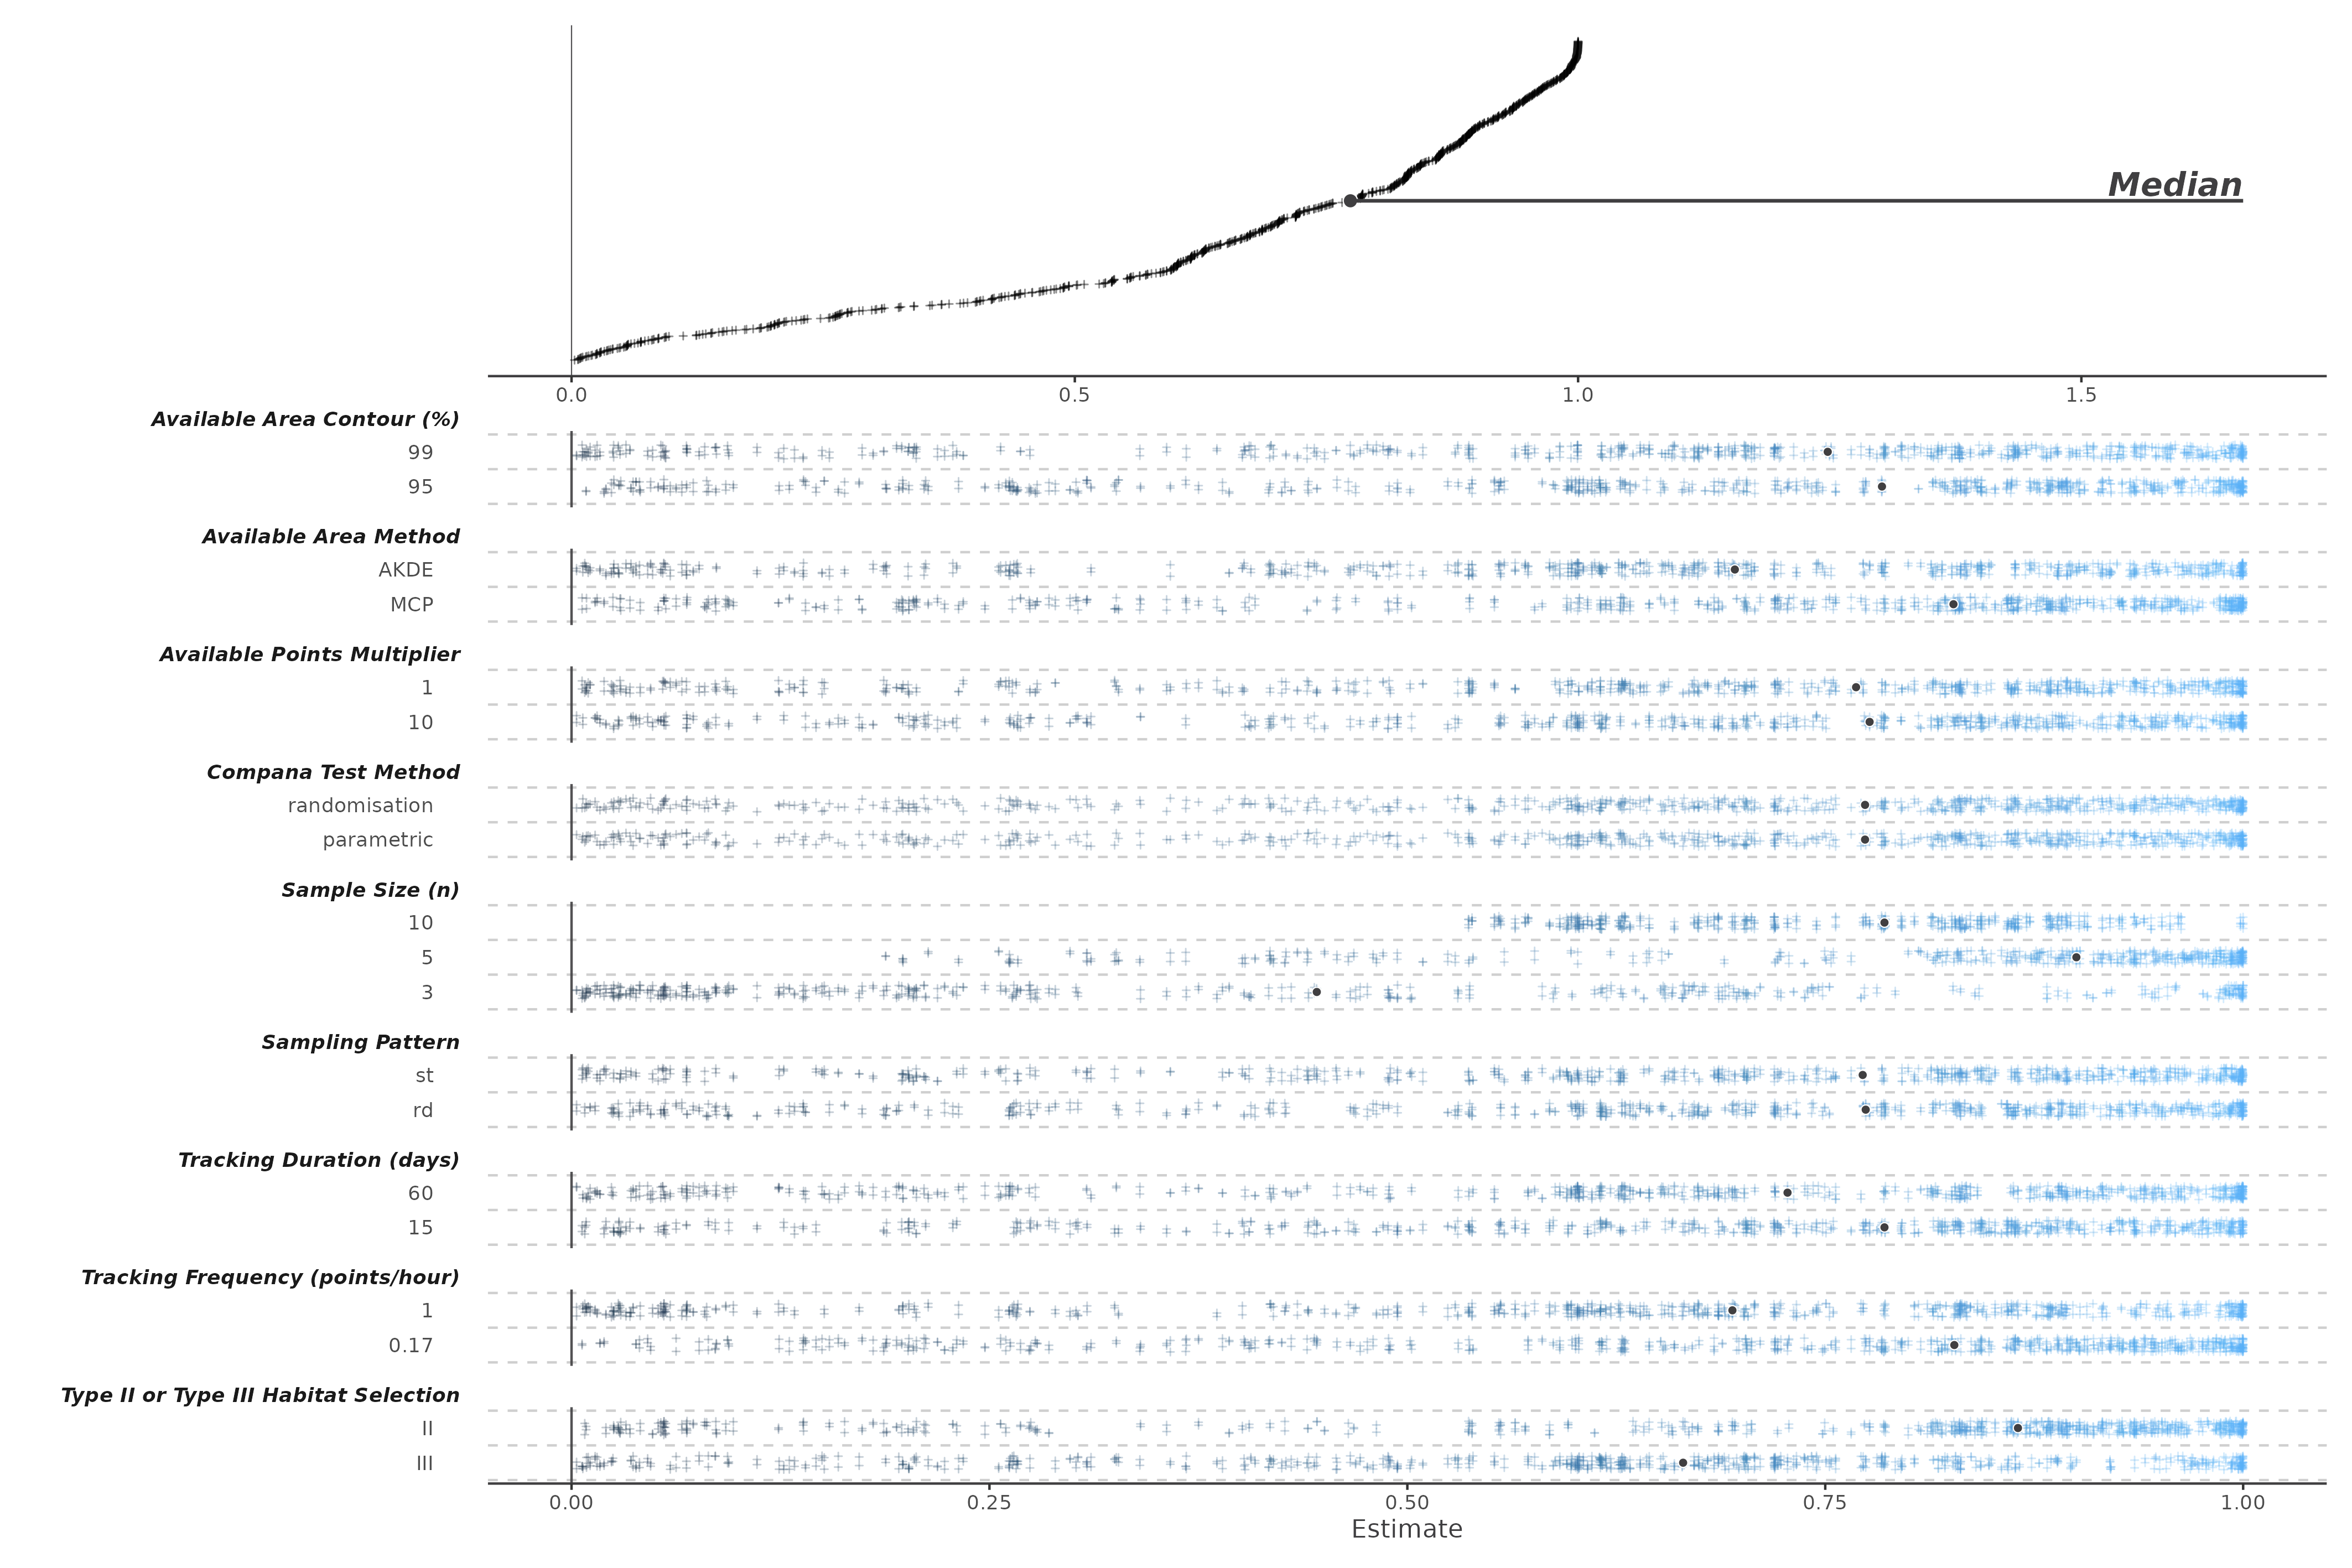
\includegraphics[width=1\linewidth]{../figures/area_specCurve} \caption{Spec curve}\label{fig:specCurveArea}
\end{figure}

(Fig. \ref{fig:specCurveSSF}).

\begin{figure}
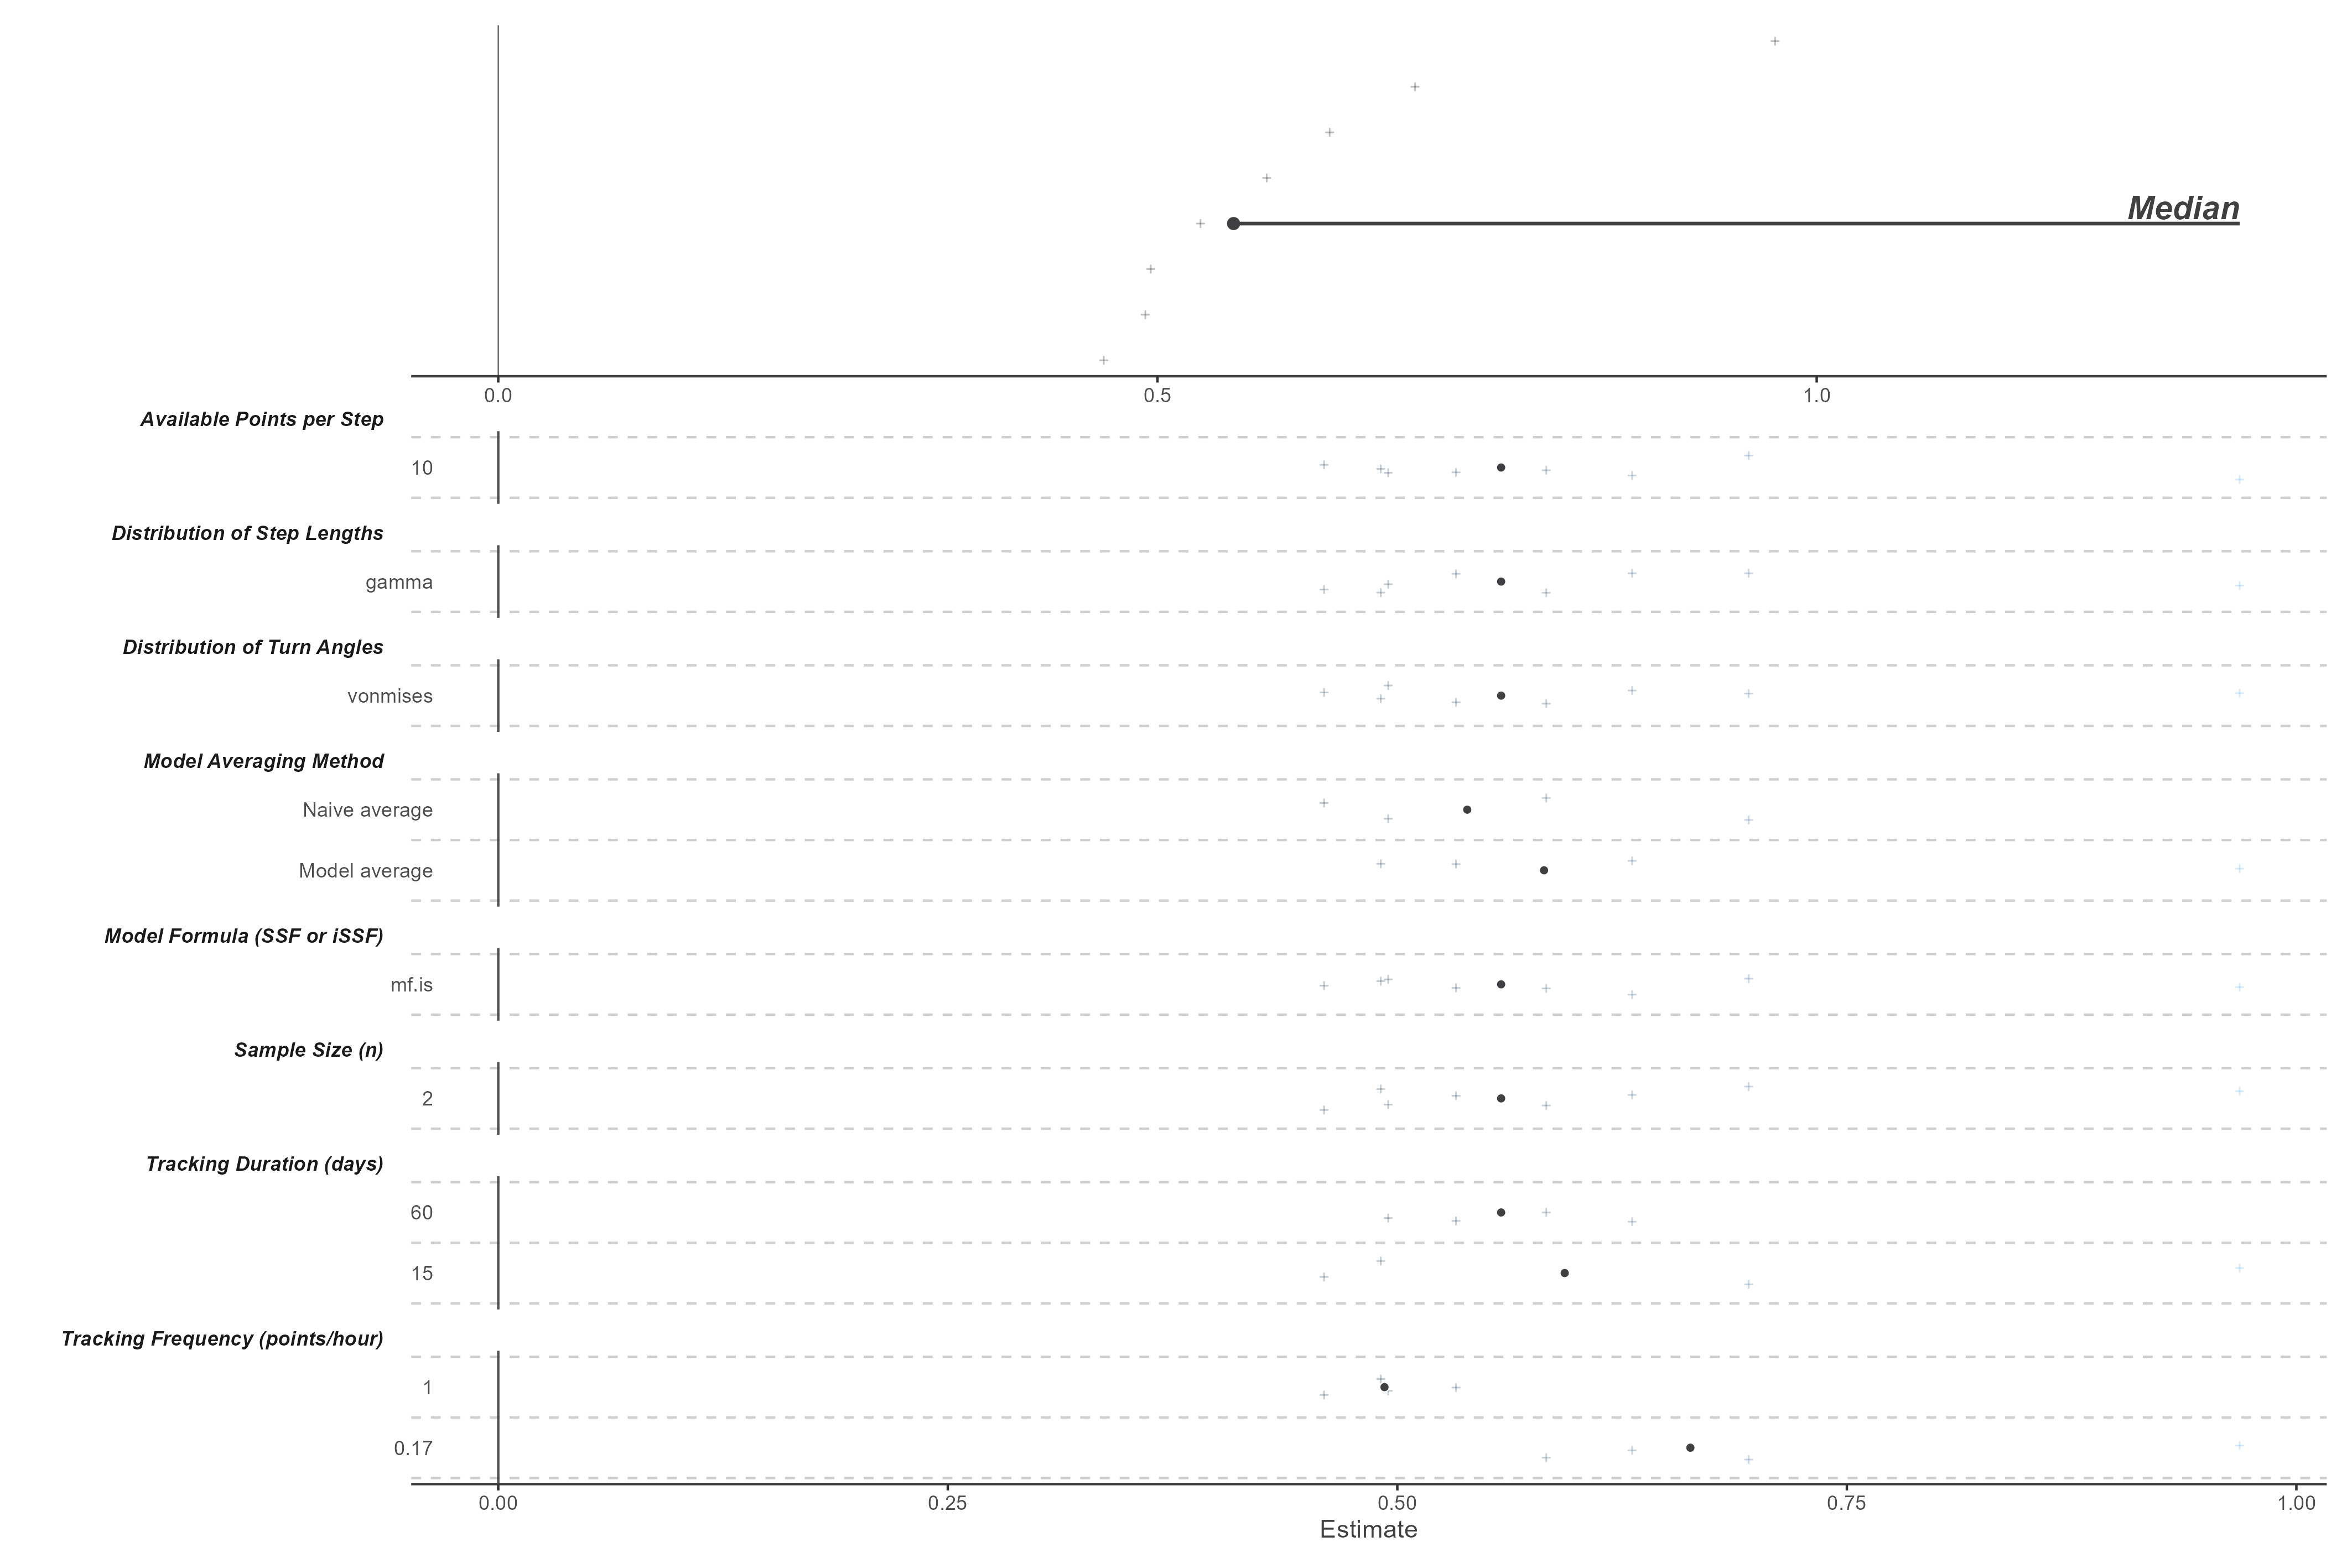
\includegraphics[width=1\linewidth]{../figures/ssf_specCurve} \caption{Spec curve}\label{fig:specCurveSSF}
\end{figure}

(Fig. \ref{fig:specCurvePois}).

\begin{figure}
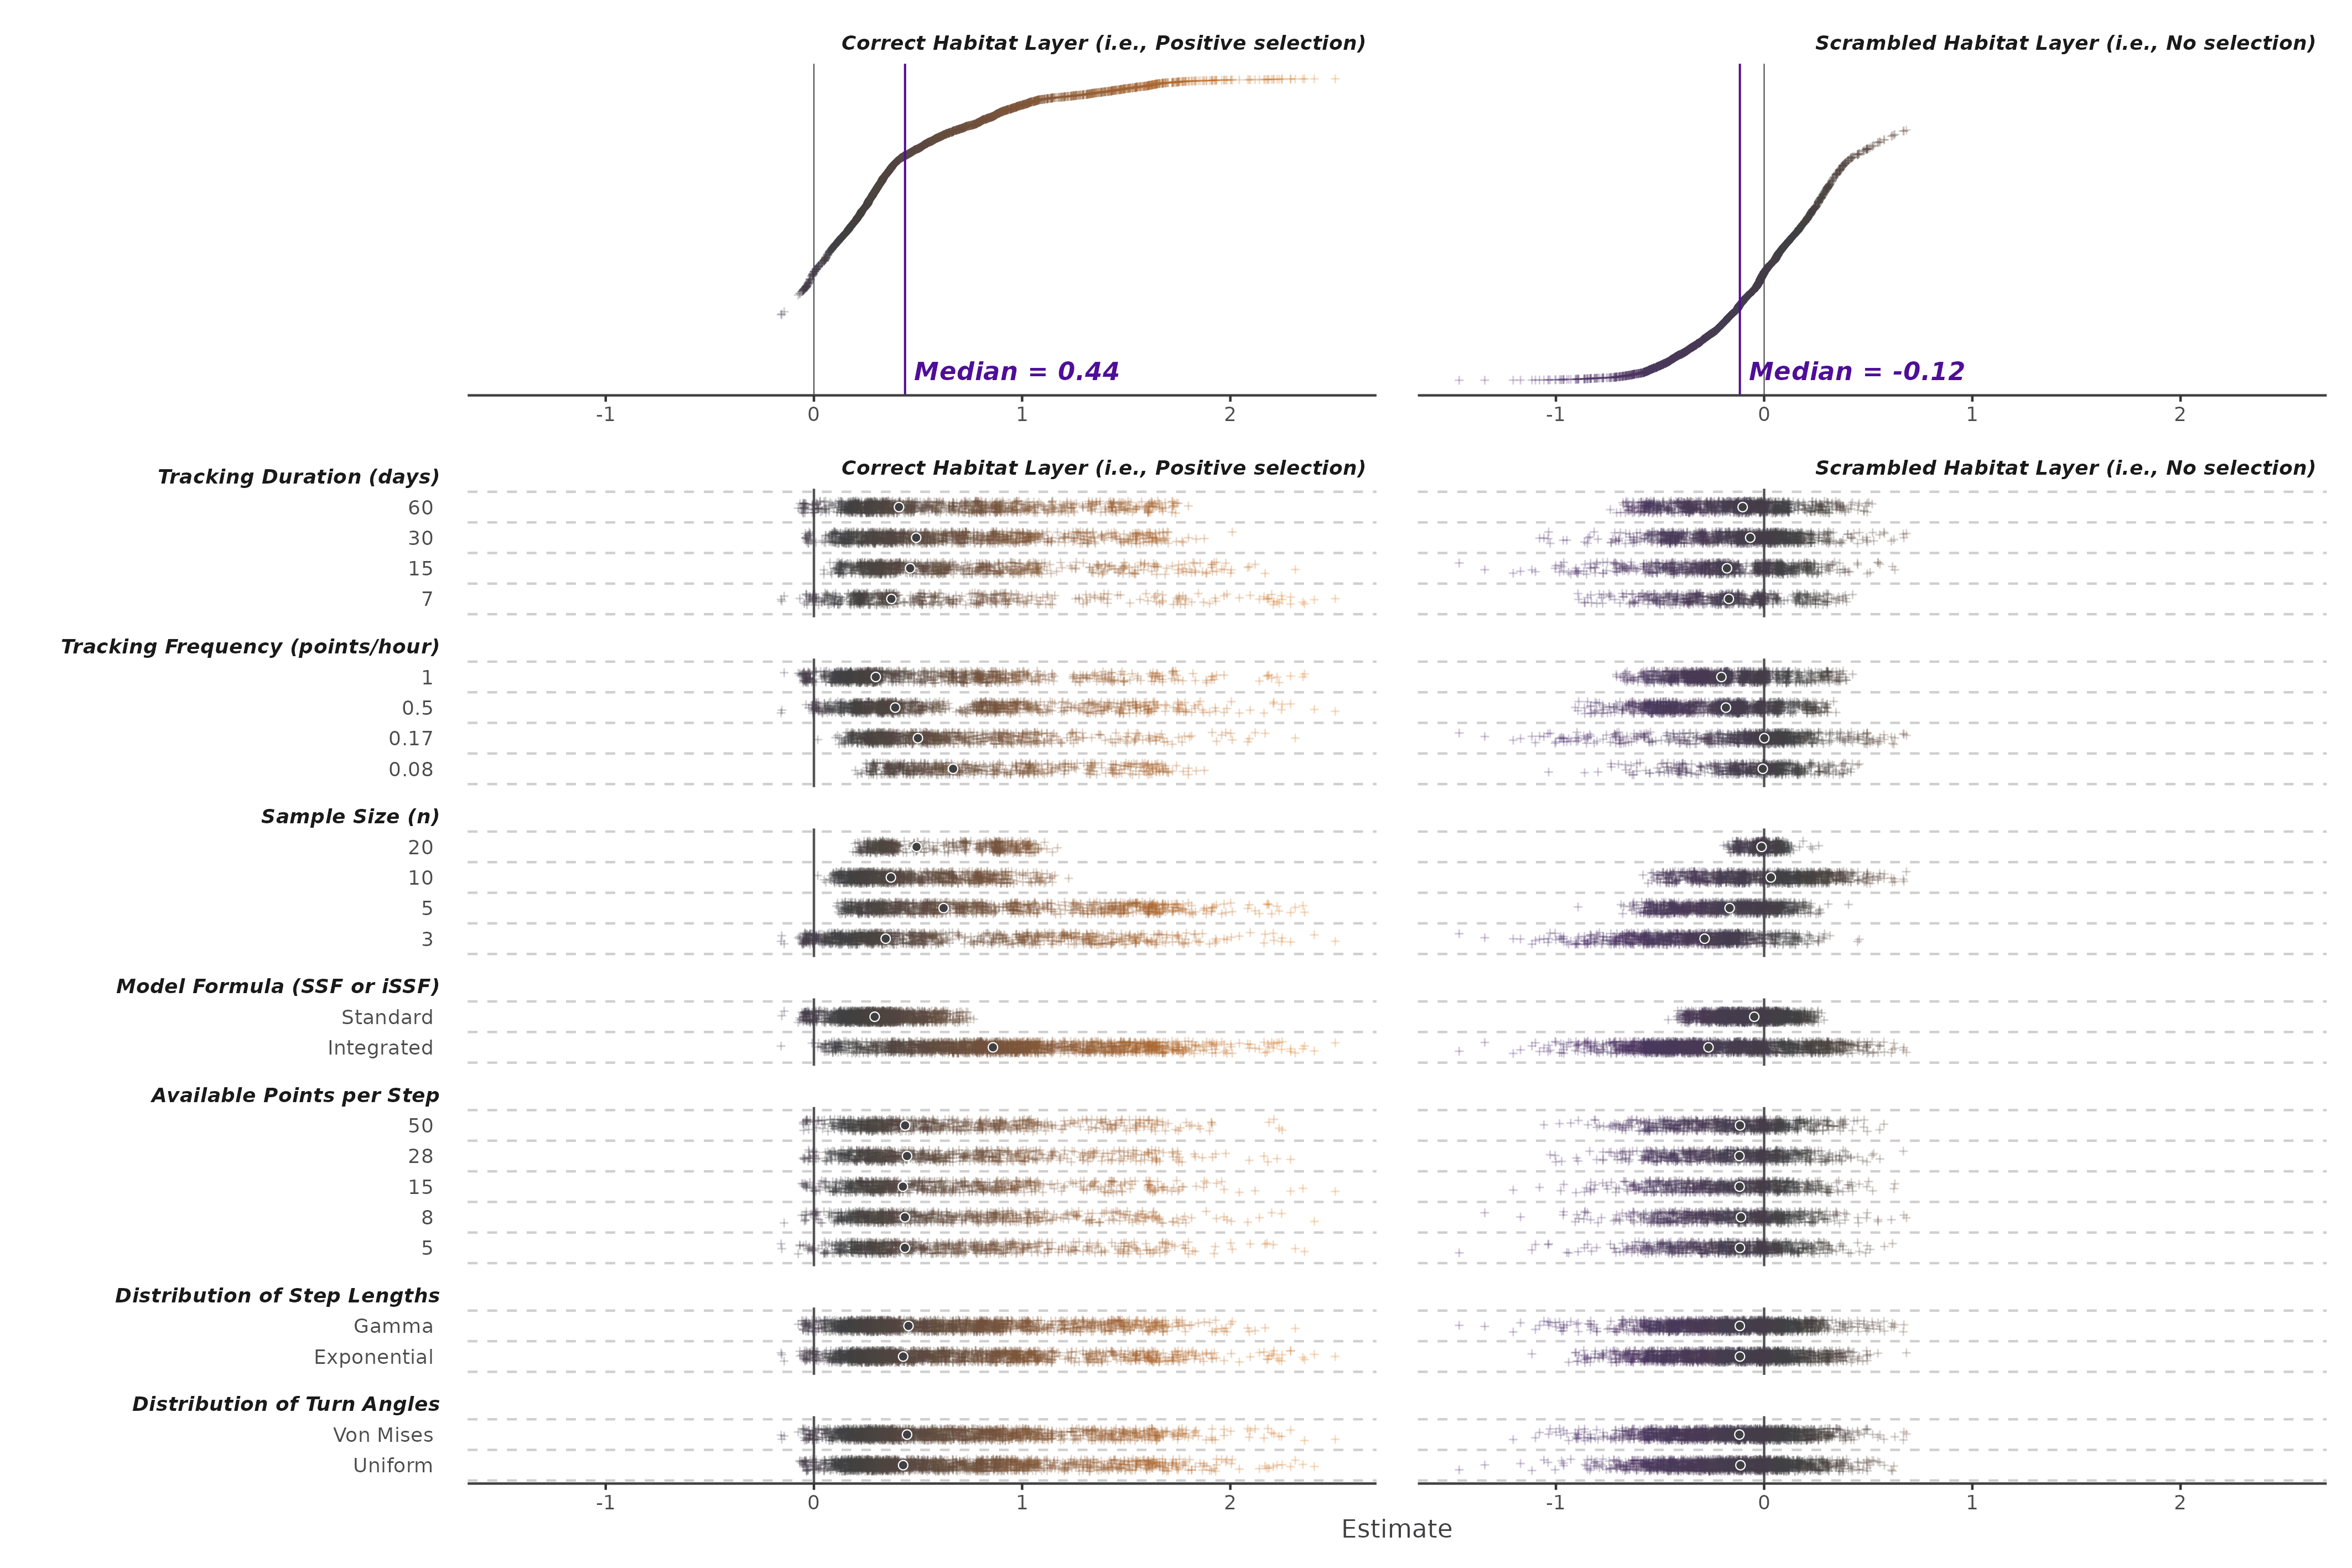
\includegraphics[width=1\linewidth]{../figures/pois_specCurve} \caption{Spec curve}\label{fig:specCurvePois}
\end{figure}

\hypertarget{model-results}{%
\subsection{Model Results}\label{model-results}}

The conditional \emph{R\textsuperscript{2}} values differed for the three models. The Compana results model had a conditional \emph{R\textsuperscript{2}} of 0.33; whereas the SSF model returned 0.59, and the Poisson model returned 0.94.

The marginal \emph{R\textsuperscript{2}} represents the bulk of the conditional \emph{R\textsuperscript{2}} suggesting an important role for the fixed/population effects. The Compana results model had a conditional \emph{R\textsuperscript{2}} of 0.48; whereas the SSF model returned 0.51, and the Poisson model returned 0.83.

The sample size was negatively correlated with deviation from the median estimate (\(\beta\) -0.03; 95\% HDCI -1.15 - 1.8).

(Fig. \ref{fig:effectPlotArea}).

\begin{figure}
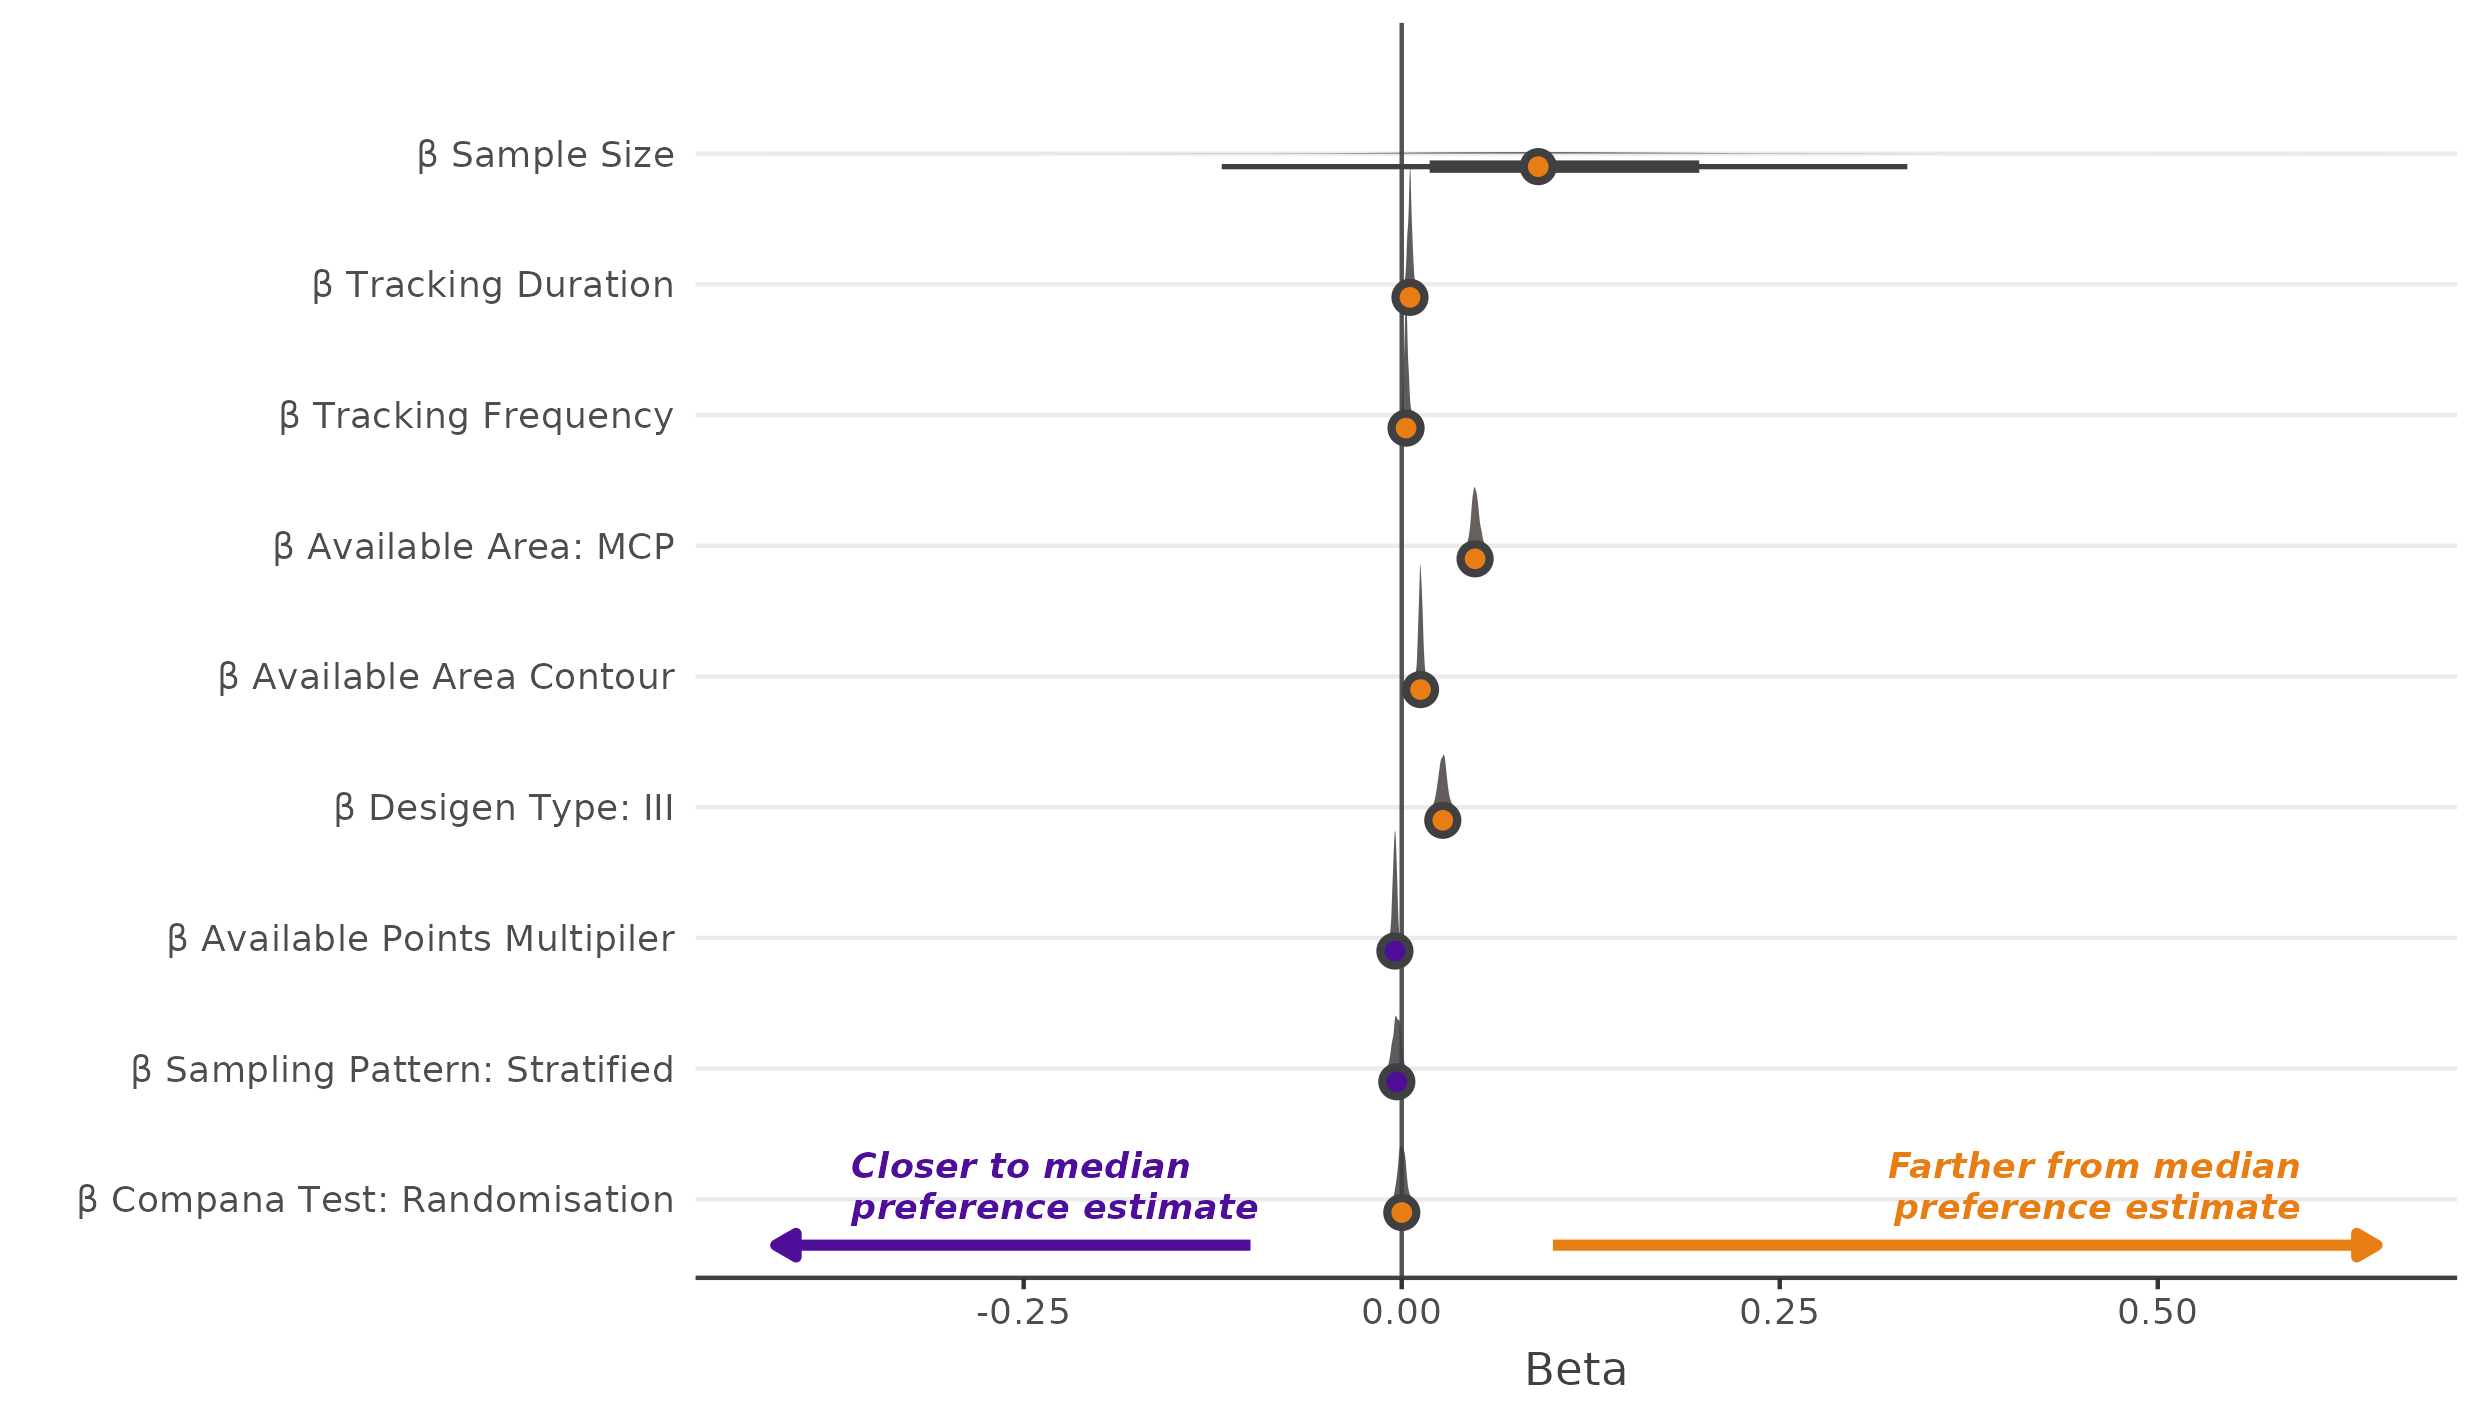
\includegraphics[width=1\linewidth]{../figures/areaBrms_effectsPlot} \caption{Beta coefs}\label{fig:effectPlotArea}
\end{figure}

(Fig. \ref{fig:effectPlotSSF}).

\begin{figure}
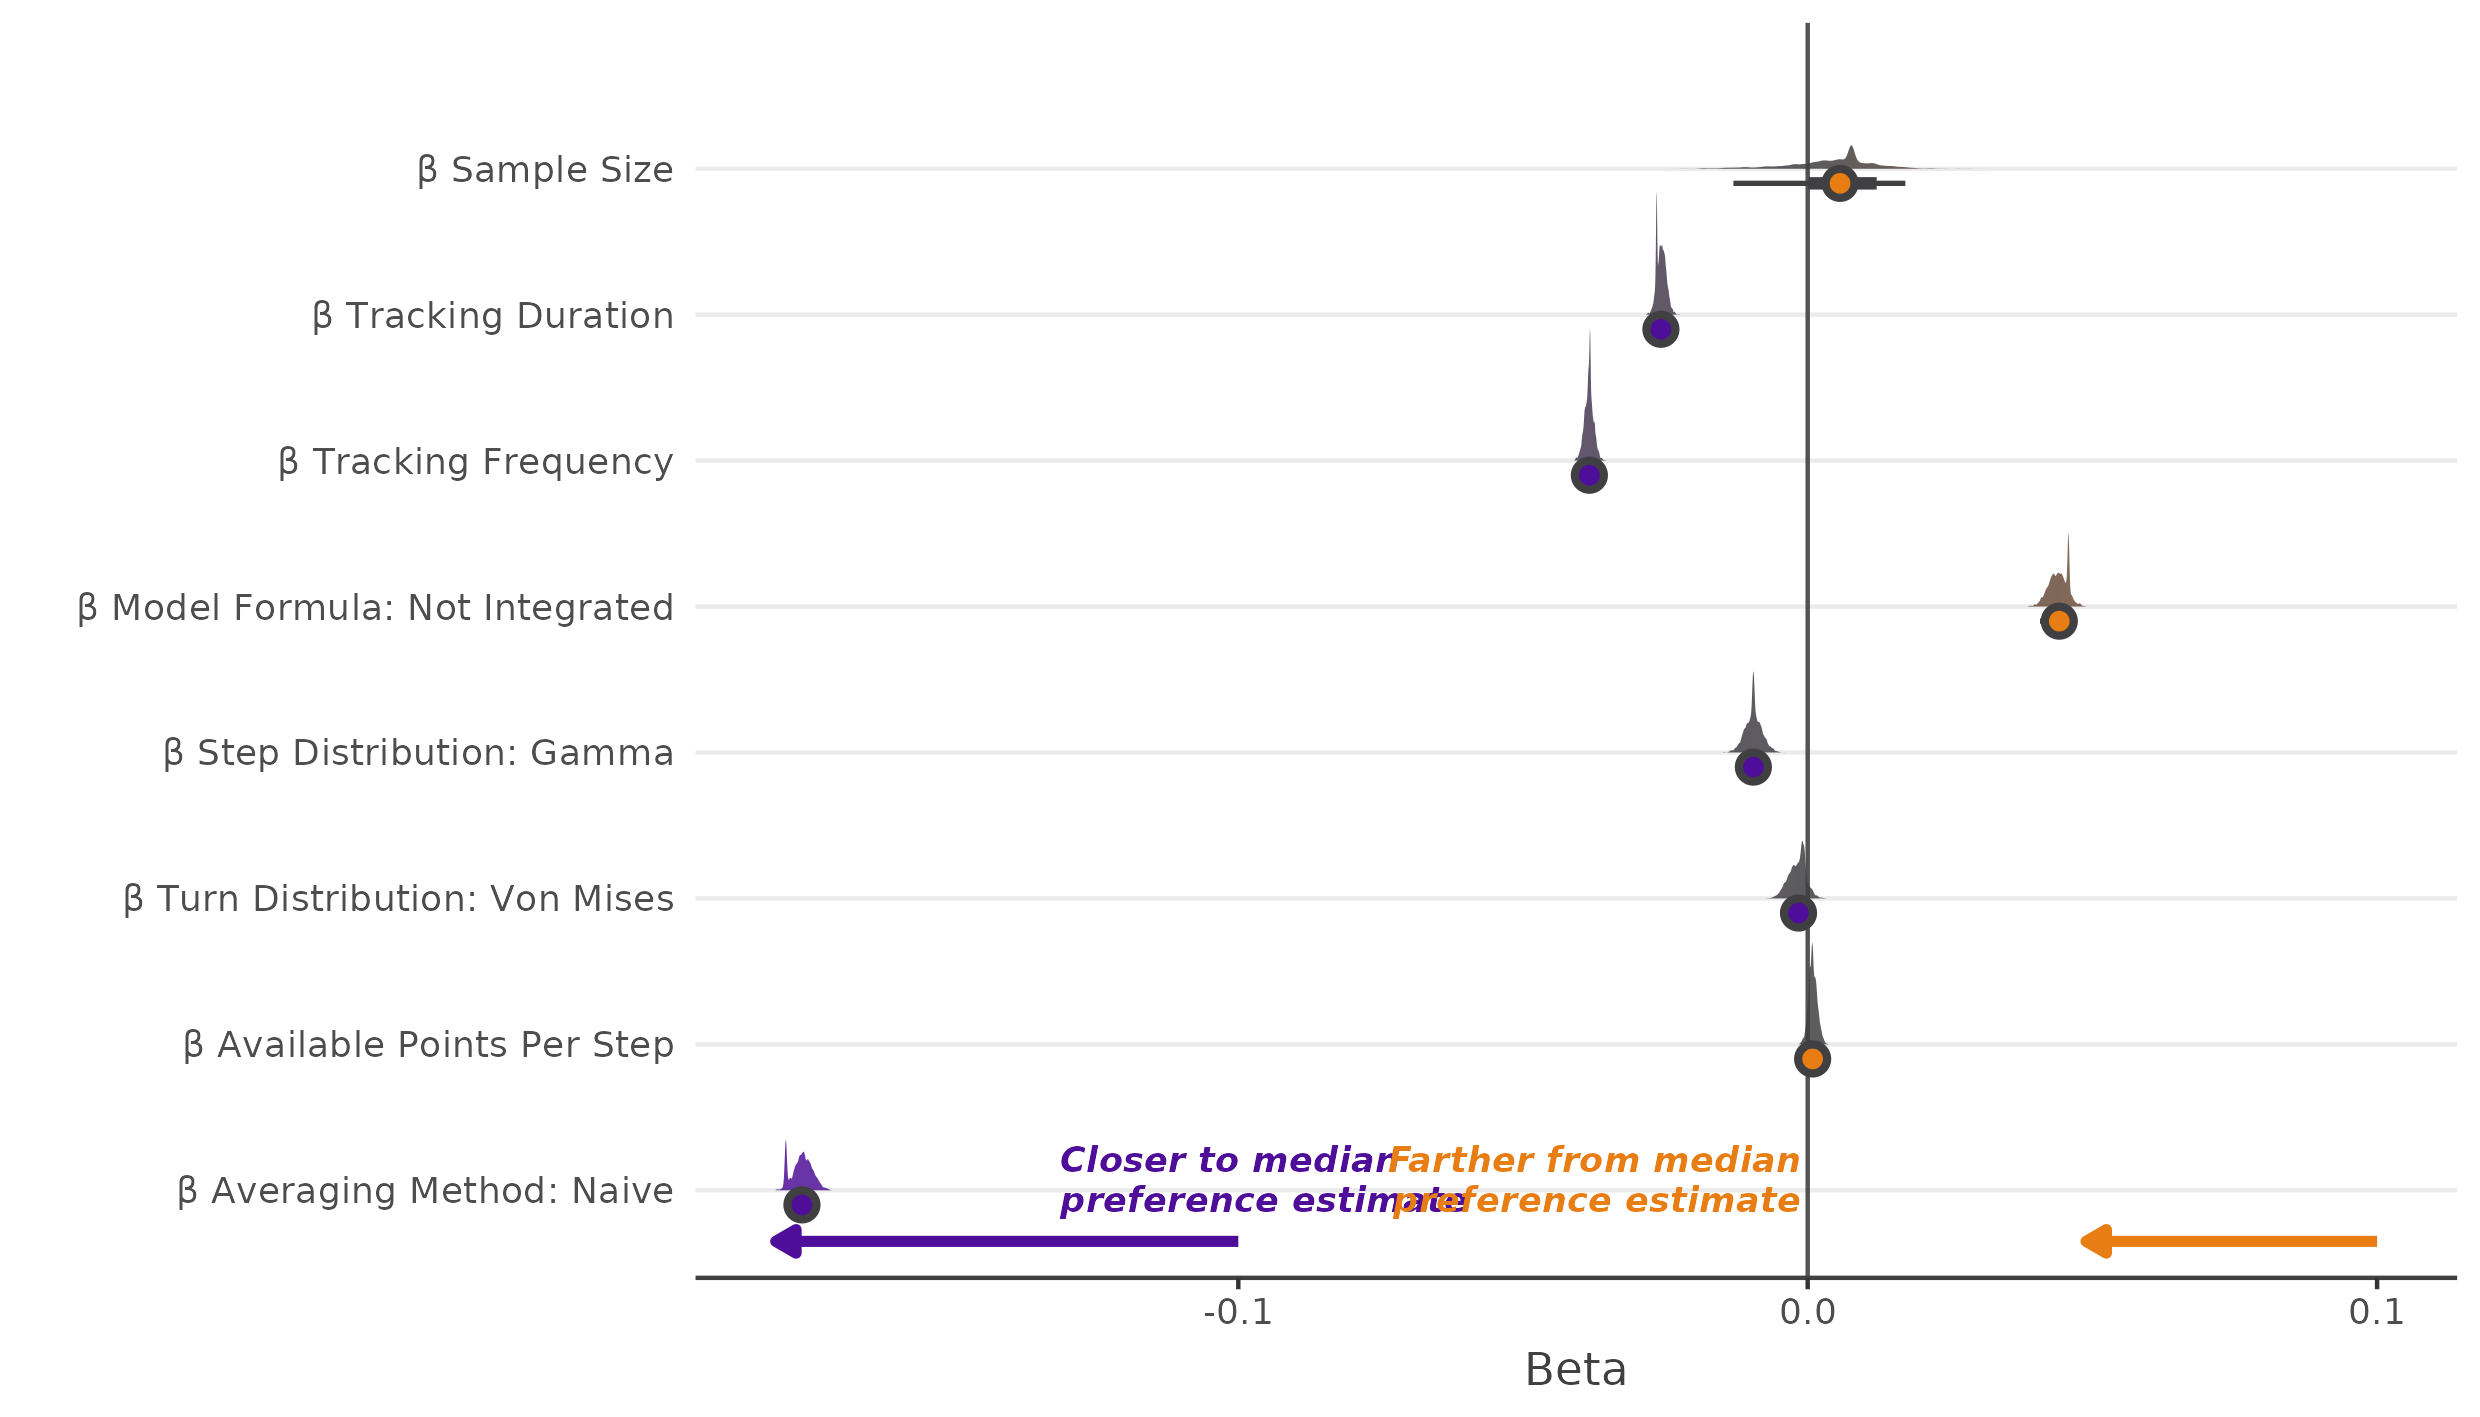
\includegraphics[width=1\linewidth]{../figures/ssfBrms_effectsPlot} \caption{Beta coefs}\label{fig:effectPlotSSF}
\end{figure}

(Fig. \ref{fig:effectPlotPois}).

\begin{figure}
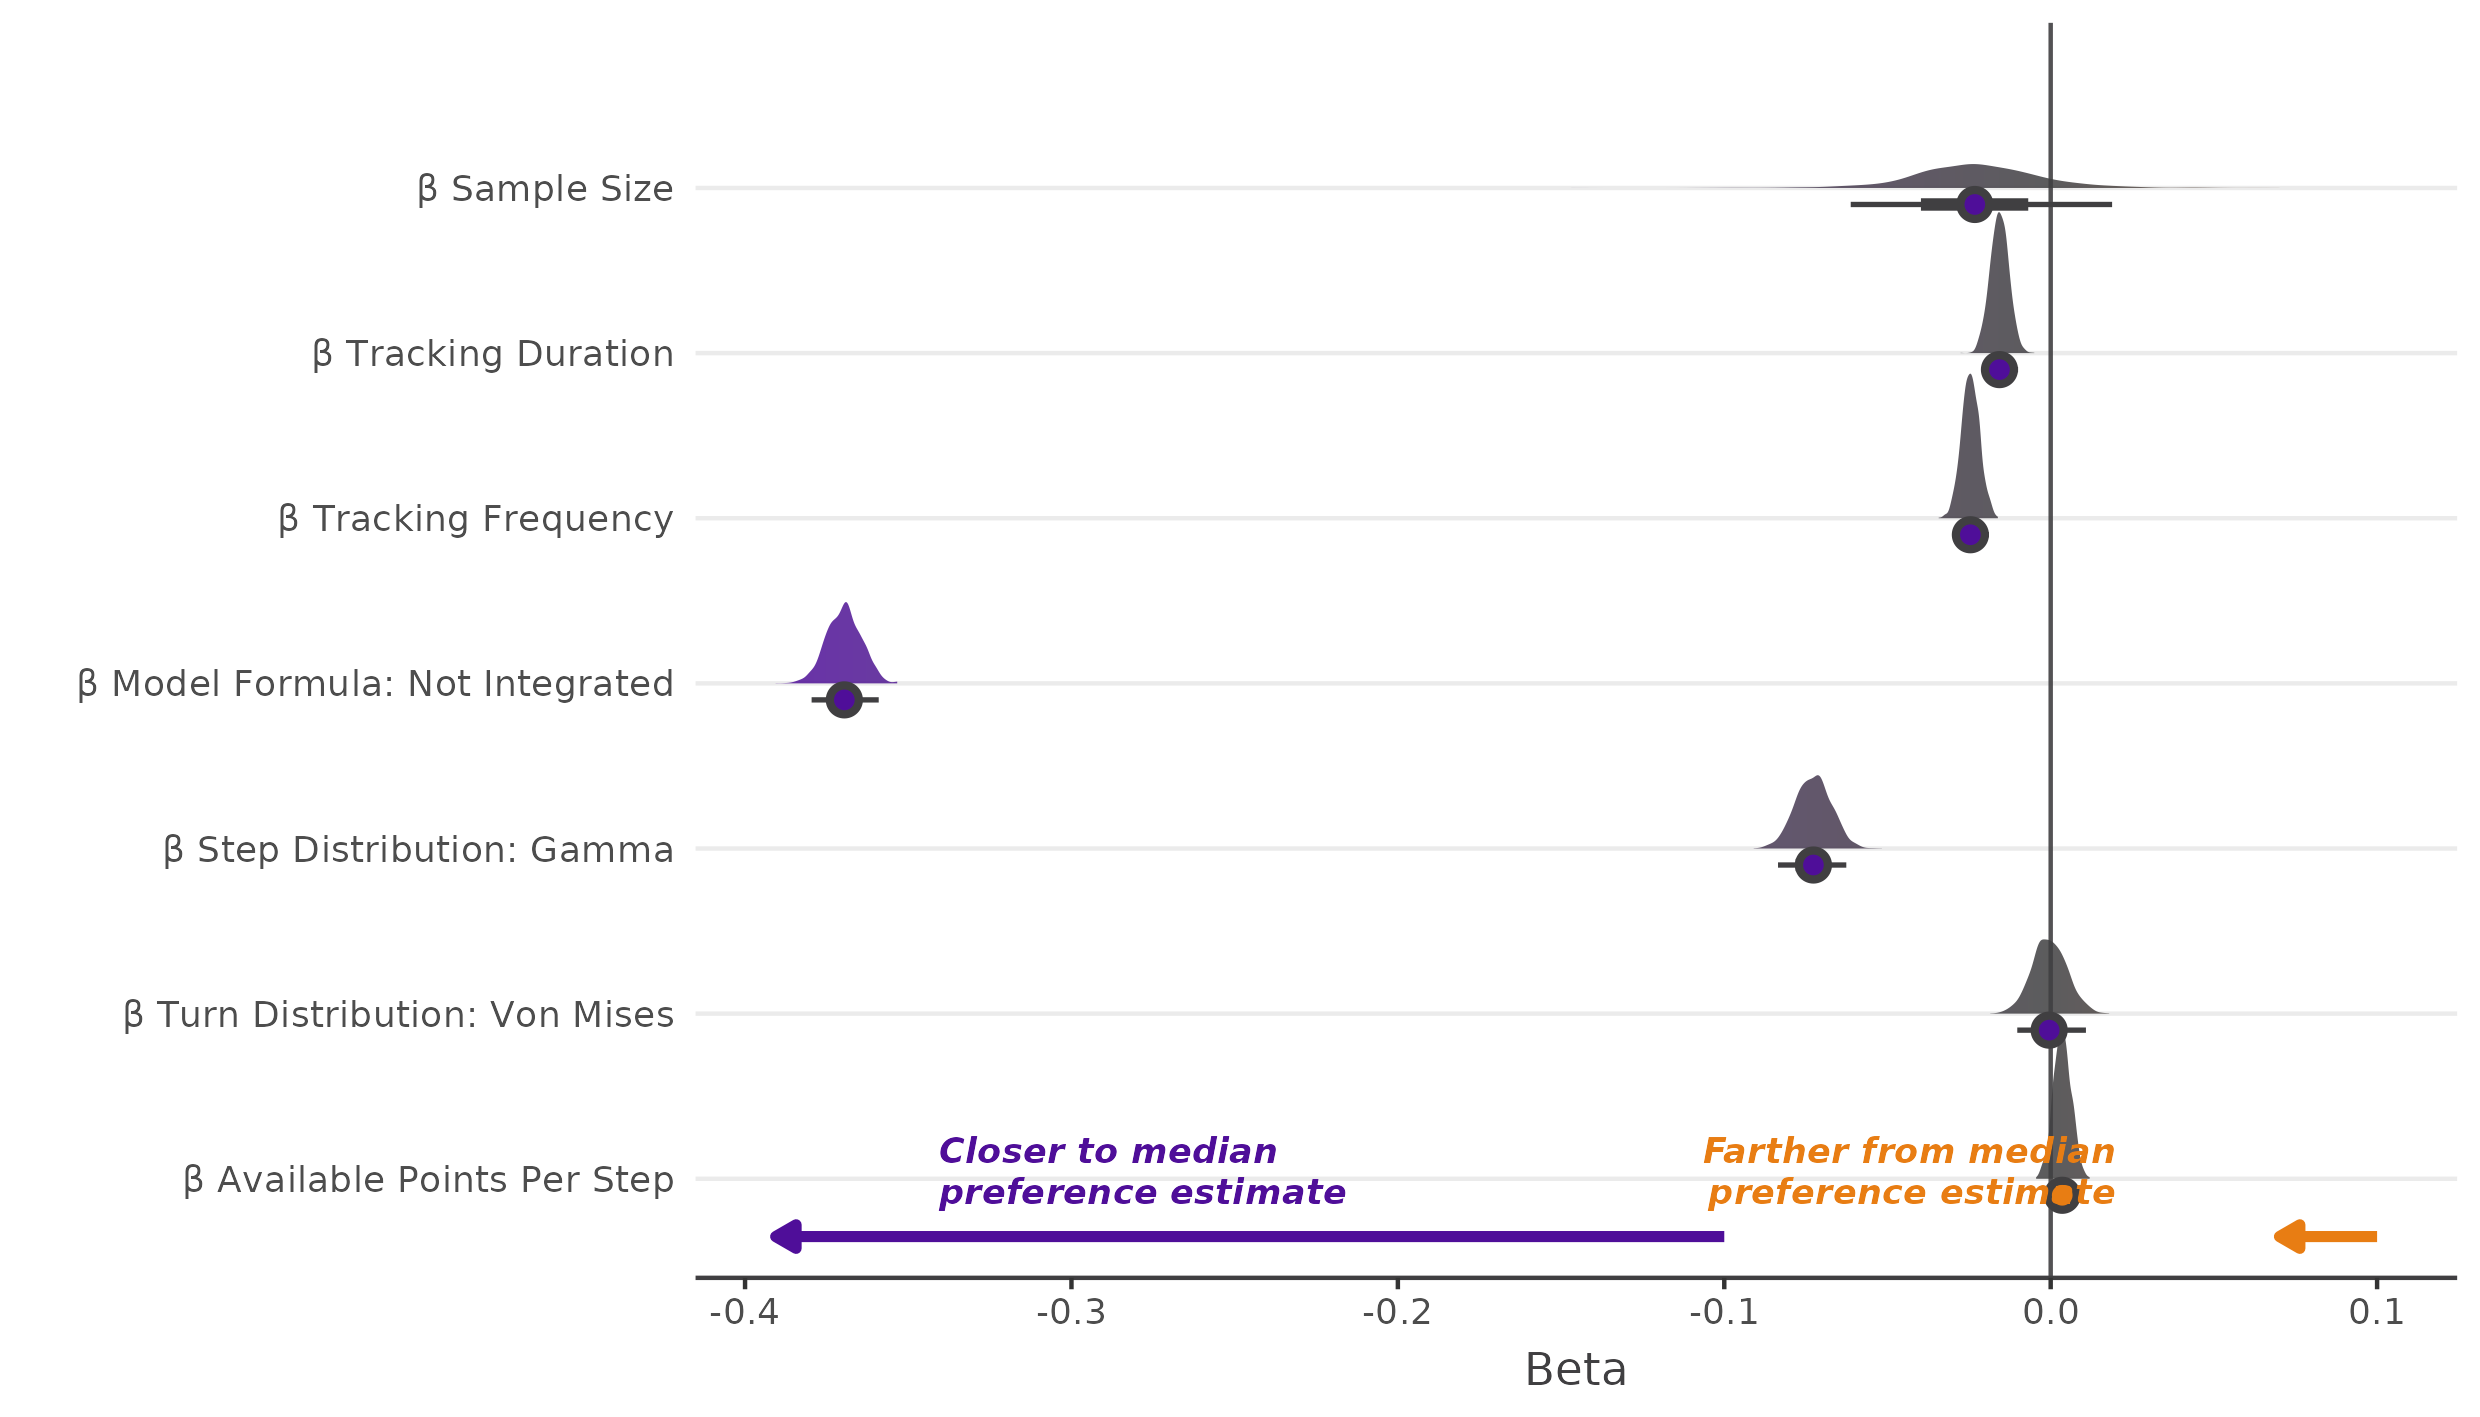
\includegraphics[width=1\linewidth]{../figures/poisBrms_effectsPlot} \caption{Beta coefs}\label{fig:effectPlotPois}
\end{figure}

\hypertarget{discussion}{%
\section{Discussion}\label{discussion}}

\hypertarget{limitations}{%
\subsection{Limitations}\label{limitations}}

\hypertarget{conclusions}{%
\subsection{Conclusions}\label{conclusions}}

\hypertarget{acknowledgements}{%
\section{Acknowledgements}\label{acknowledgements}}

BMM was funded by the Natural Environment Research Council (NERC) via the IAPETUS2 Doctoral Training Partnership.

\hypertarget{software-availablity}{%
\section{Software availablity}\label{software-availablity}}

In addition to packages already mentioned in the methods we also used the following.

We used \emph{R} v.4.2.2 (\protect\hyperlink{ref-base}{R Core Team, 2023}) via \emph{RStudio} v.2023.6.2.561 (\protect\hyperlink{ref-rstudio}{RStudio Team, 2022}).
We used \emph{here} v.1.0.1 (\protect\hyperlink{ref-here}{Müller, 2020}) and \emph{qs} v.0.25.5 (\protect\hyperlink{ref-qs}{Ching, 2023}) to manage directory addresses and saved objects.

We used \emph{raster} v.3.6.14 (\protect\hyperlink{ref-raster}{Hijmans, 2023}) and \emph{RandomFields} v.3.3.14 (\protect\hyperlink{ref-RandomFields}{Schlather et al., 2015}) to aid landscape raster creation alongside NLMR v.1.1.1 (\protect\hyperlink{ref-NLMR}{Sciaini et al., 2018}).

We used \emph{ggplot2} v.3.4.2 for creating figures (\protect\hyperlink{ref-ggplot2}{Wickham, 2016}), with the expansions: \emph{patchwork} v.1.1.2 (\protect\hyperlink{ref-patchwork}{Pedersen, 2022}), \emph{ggridges} v.0.5.4 (\protect\hyperlink{ref-ggridges}{Wilke, 2022}), and \emph{ggdist} v.3.2.0 (\protect\hyperlink{ref-ggdist}{Kay, 2023a}).

We used \emph{brms} v.2.19.0 (\protect\hyperlink{ref-brms}{Bürkner, 2021}) to run Bayesian models, with dianogistics generated used \emph{bayesplot} v.1.10.0 (\protect\hyperlink{ref-bayesplot}{Gabry et al., 2019}), \emph{tidybayes} v.3.0.2 (\protect\hyperlink{ref-tidybayes}{Kay, 2023b}), and \emph{performance} v.0.10.2 (\protect\hyperlink{ref-performance}{Lüdecke et al., 2021}).

We used the \emph{dplyr} v.1.0.10 (\protect\hyperlink{ref-dplyr}{Wickham et al., 2023}), \emph{tibble} v.3.1.8 (\protect\hyperlink{ref-tibble}{Müller \& Wickham, 2023}),
and \emph{stringr} v.1.5.0 (\protect\hyperlink{ref-stringr}{Wickham, 2022}) packages for data manipulation.

We used \emph{sp} v.1.5.1 (\protect\hyperlink{ref-sp}{Bivand, Pebesma \& Gomez-Rubio, 2013}), \emph{adehabitatHR} v.0.4.20 (\protect\hyperlink{ref-adehabitatHR}{Calenge \& Scott Fortmann-Roe, 2023}), \emph{move} v.4.1.12 (\protect\hyperlink{ref-move}{Kranstauber, Smolla \& Scharf, 2023}) for manipulation of spatial data and estimation of space use not otherwise mentioned in the methods.

We used rmarkdown v.2.19 (\protect\hyperlink{ref-rmarkdown2018}{Xie, Allaire \& Grolemund, 2018}; \protect\hyperlink{ref-rmarkdown2020}{Xie, Dervieux \& Riederer, 2020}; \protect\hyperlink{ref-rmarkdown2023}{Allaire et al., 2023}), bookdown v.0.33 (\protect\hyperlink{ref-bookdown2016}{Xie, 2016}, \protect\hyperlink{ref-R-bookdown}{2022}), tinytex v.0.44 (\protect\hyperlink{ref-tinytex2019}{Xie, 2019}, \protect\hyperlink{ref-tinytex2023}{2023a}), and knitr v.1.41 (\protect\hyperlink{ref-knitr2014}{Xie, 2014}, \protect\hyperlink{ref-knitr2015}{2015}, \protect\hyperlink{ref-knitr2023}{2023b}) packages to generate type-set outputs.

We generated R package citations with the aid of \emph{grateful} v.0.1.13 (\protect\hyperlink{ref-grateful}{Francisco Rodríguez-Sánchez, Connor P. Jackson \& Shaurita D. Hutchins, 2023}).

\hypertarget{data-availabilty}{%
\section{Data availabilty}\label{data-availabilty}}

\hypertarget{supplementary-material}{%
\section{Supplementary Material}\label{supplementary-material}}

\hypertarget{references}{%
\section*{References}\label{references}}
\addcontentsline{toc}{section}{References}

\hypertarget{refs}{}
\begin{CSLReferences}{1}{0}
\leavevmode\vadjust pre{\hypertarget{ref-rmarkdown2023}{}}%
Allaire J, Xie Y, Dervieux C, McPherson J, Luraschi J, Ushey K, Atkins A, Wickham H, Cheng J, Chang W, Iannone R. 2023. \emph{\href{https://github.com/rstudio/rmarkdown}{{rmarkdown}: Dynamic documents for r}}.

\leavevmode\vadjust pre{\hypertarget{ref-sp}{}}%
Bivand RS, Pebesma E, Gomez-Rubio V. 2013. \emph{\href{https://asdar-book.org/}{Applied spatial data analysis with {R}, second edition}}. Springer, NY.

\leavevmode\vadjust pre{\hypertarget{ref-brms}{}}%
Bürkner P-C. 2021. Bayesian item response modeling in {R} with {brms} and {Stan}. \emph{Journal of Statistical Software} 100:1--54. DOI: \href{https://doi.org/10.18637/jss.v100.i05}{10.18637/jss.v100.i05}.

\leavevmode\vadjust pre{\hypertarget{ref-adehabitatHS}{}}%
Calenge C, Mathieu Basille contributions from. 2023. \emph{\href{https://CRAN.R-project.org/package=adehabitatHS}{{adehabitatHS}: Analysis of habitat selection by animals}}.

\leavevmode\vadjust pre{\hypertarget{ref-adehabitatHR}{}}%
Calenge C, Scott Fortmann-Roe contributions from. 2023. \emph{\href{https://CRAN.R-project.org/package=adehabitatHR}{{adehabitatHR}: Home range estimation}}.

\leavevmode\vadjust pre{\hypertarget{ref-qs}{}}%
Ching T. 2023. \emph{\href{https://CRAN.R-project.org/package=qs}{{qs}: Quick serialization of r objects}}.

\leavevmode\vadjust pre{\hypertarget{ref-ctmm}{}}%
Fleming CH, Calabrese JM. 2023. \emph{{ctmm}: Continuous-time movement modeling}.

\leavevmode\vadjust pre{\hypertarget{ref-grateful}{}}%
Francisco Rodríguez-Sánchez, Connor P. Jackson, Shaurita D. Hutchins. 2023. \emph{\href{https://github.com/Pakillo/grateful}{{grateful}: Facilitate citation of r packages}}.

\leavevmode\vadjust pre{\hypertarget{ref-bayesplot}{}}%
Gabry J, Simpson D, Vehtari A, Betancourt M, Gelman A. 2019. Visualization in bayesian workflow. \emph{J. R. Stat. Soc. A} 182:389--402. DOI: \href{https://doi.org/10.1111/rssa.12378}{10.1111/rssa.12378}.

\leavevmode\vadjust pre{\hypertarget{ref-raster}{}}%
Hijmans RJ. 2023. \emph{\href{https://CRAN.R-project.org/package=raster}{{raster}: Geographic data analysis and modeling}}.

\leavevmode\vadjust pre{\hypertarget{ref-ggdist}{}}%
Kay M. 2023a. \emph{{ggdist}: Visualizations of distributions and uncertainty}. DOI: \href{https://doi.org/10.5281/zenodo.3879620}{10.5281/zenodo.3879620}.

\leavevmode\vadjust pre{\hypertarget{ref-tidybayes}{}}%
Kay M. 2023b. \emph{{tidybayes}: Tidy data and geoms for {Bayesian} models}. DOI: \href{https://doi.org/10.5281/zenodo.1308151}{10.5281/zenodo.1308151}.

\leavevmode\vadjust pre{\hypertarget{ref-kourounis_towards_2018}{}}%
Kourounis D, Fuchs A, Schenk O. 2018. \href{https://doi.org/10.1109/TPWRS.2017.2789187}{Towards the next generation of multiperiod optimal power flow solvers}. \emph{IEEE Transactions on Power Systems} PP:1--10.

\leavevmode\vadjust pre{\hypertarget{ref-move}{}}%
Kranstauber B, Smolla M, Scharf AK. 2023. \emph{\href{https://CRAN.R-project.org/package=move}{{move}: Visualizing and analyzing animal track data}}.

\leavevmode\vadjust pre{\hypertarget{ref-tarchetypes}{}}%
Landau WM. 2021b. \emph{Tarchetypes: Archetypes for targets}.

\leavevmode\vadjust pre{\hypertarget{ref-targets}{}}%
Landau WM. 2021a. \href{https://doi.org/10.21105/joss.02959}{The targets r package: A dynamic make-like function-oriented pipeline toolkit for reproducibility and high-performance computing}. \emph{Journal of Open Source Software} 6:2959.

\leavevmode\vadjust pre{\hypertarget{ref-lindgren_explicit_2011}{}}%
Lindgren F, Rue H, Lindström J. 2011. An explicit link between {Gaussian} fields and {Gaussian} {Markov} random fields: The stochastic partial differential equation approach (with discussion). \emph{Journal of the Royal Statistical Society B} 73:423--498.

\leavevmode\vadjust pre{\hypertarget{ref-performance}{}}%
Lüdecke D, Ben-Shachar MS, Patil I, Waggoner P, Makowski D. 2021. {performance}: An {R} package for assessment, comparison and testing of statistical models. \emph{Journal of Open Source Software} 6:3139. DOI: \href{https://doi.org/10.21105/joss.03139}{10.21105/joss.03139}.

\leavevmode\vadjust pre{\hypertarget{ref-abmAnimalMovement}{}}%
Marshall BM, Duthie AB. 2022. \href{https://0}{{abmAnimalMovement}: An r package for simulating animal movement using an agent-based model}. \emph{F1000} 0:0.

\leavevmode\vadjust pre{\hypertarget{ref-martins_bayesian_2013}{}}%
Martins TG, Simpson D, Lindgren F, Rue H. 2013. Bayesian computing with {INLA}: {N}ew features. \emph{Computational Statistics and Data Analysis} 67:68--83.

\leavevmode\vadjust pre{\hypertarget{ref-muff_accounting_2020}{}}%
Muff S, Signer J, Fieberg J. 2020. Accounting for individual-specific variation in habitat-selection studies: Efficient estimation of mixed-effects models using bayesian or frequentist computation. \emph{Journal of Animal Ecology} 89:80--92. DOI: \href{https://doi.org/10.1111/1365-2656.13087}{10.1111/1365-2656.13087}.

\leavevmode\vadjust pre{\hypertarget{ref-here}{}}%
Müller K. 2020. \emph{\href{https://CRAN.R-project.org/package=here}{{here}: A simpler way to find your files}}.

\leavevmode\vadjust pre{\hypertarget{ref-tibble}{}}%
Müller K, Wickham H. 2023. \emph{\href{https://CRAN.R-project.org/package=tibble}{{tibble}: Simple data frames}}.

\leavevmode\vadjust pre{\hypertarget{ref-patchwork}{}}%
Pedersen TL. 2022. \emph{\href{https://CRAN.R-project.org/package=patchwork}{Patchwork: The composer of plots}}.

\leavevmode\vadjust pre{\hypertarget{ref-base}{}}%
R Core Team. 2023. \emph{\href{https://www.R-project.org/}{R: A language and environment for statistical computing}}. Vienna, Austria: R Foundation for Statistical Computing.

\leavevmode\vadjust pre{\hypertarget{ref-rstudio}{}}%
RStudio Team. 2022. \emph{\href{http://www.rstudio.com/}{{RStudio}: Integrated development environment for r}}. Boston, MA: RStudio, PBC.

\leavevmode\vadjust pre{\hypertarget{ref-rue_approximate_2009}{}}%
Rue H, Martino S, Chopin N. 2009. Approximate {Bayesian} inference for latent {Gaussian} models using integrated nested {Laplace} approximations (with discussion). \emph{Journal of the Royal Statistical Society B} 71:319--392.

\leavevmode\vadjust pre{\hypertarget{ref-rue_bayesian_2017}{}}%
Rue H, Riebler AI, Sørbye SH, Illian JB, Simpson DP, Lindgren FK. 2017. \href{http://arxiv.org/abs/1604.00860}{Bayesian computing with {INLA}: {A} review}. \emph{Annual Reviews of Statistics and Its Applications} 4:395--421.

\leavevmode\vadjust pre{\hypertarget{ref-RandomFields}{}}%
Schlather M, Malinowski A, Menck PJ, Oesting M, Strokorb K. 2015. \href{https://www.jstatsoft.org/v63/i08/}{Analysis, simulation and prediction of multivariate random fields with package {RandomFields}}. \emph{Journal of Statistical Software} 63:1--25.

\leavevmode\vadjust pre{\hypertarget{ref-NLMR}{}}%
Sciaini M, Fritsch M, Scherer C, Simpkins CE. 2018. \href{https://doi.org/10.1111/2041-210X.13076}{NLMR and landscapetools: An integrated environment for simulating and modifying neutral landscape models in r}. \emph{Methods in Ecololgy and Evolution} 00:1--9.

\leavevmode\vadjust pre{\hypertarget{ref-amt}{}}%
Signer J, Fieberg J, Avgar T. 2019. Animal movement tools (amt): R package for managing tracking data and conducting habitat selection analyses. \emph{Ecology and Evolution} 9:880--890.

\leavevmode\vadjust pre{\hypertarget{ref-ggplot2}{}}%
Wickham H. 2016. \emph{\href{https://ggplot2.tidyverse.org}{ggplot2: Elegant graphics for data analysis}}. Springer-Verlag New York.

\leavevmode\vadjust pre{\hypertarget{ref-stringr}{}}%
Wickham H. 2022. \emph{\href{https://CRAN.R-project.org/package=stringr}{{stringr}: Simple, consistent wrappers for common string operations}}.

\leavevmode\vadjust pre{\hypertarget{ref-dplyr}{}}%
Wickham H, François R, Henry L, Müller K, Vaughan D. 2023. \emph{\href{https://CRAN.R-project.org/package=dplyr}{{dplyr}: A grammar of data manipulation}}.

\leavevmode\vadjust pre{\hypertarget{ref-ggridges}{}}%
Wilke CO. 2022. \emph{\href{https://CRAN.R-project.org/package=ggridges}{Ggridges: Ridgeline plots in 'ggplot2'}}.

\leavevmode\vadjust pre{\hypertarget{ref-knitr2014}{}}%
Xie Y. 2014. {knitr}: A comprehensive tool for reproducible research in {R}. In: Stodden V, Leisch F, Peng RD eds. \emph{Implementing reproducible computational research}. Chapman; Hall/CRC,.

\leavevmode\vadjust pre{\hypertarget{ref-knitr2015}{}}%
Xie Y. 2015. \emph{\href{https://yihui.org/knitr/}{Dynamic documents with {R} and knitr}}. Boca Raton, Florida: Chapman; Hall/CRC.

\leavevmode\vadjust pre{\hypertarget{ref-bookdown2016}{}}%
Xie Y. 2016. \emph{\href{https://bookdown.org/yihui/bookdown}{{bookdown}: Authoring books and technical documents with {R} markdown}}. Boca Raton, Florida: Chapman; Hall/CRC.

\leavevmode\vadjust pre{\hypertarget{ref-tinytex2019}{}}%
Xie Y. 2019. \href{https://tug.org/TUGboat/Contents/contents40-1.html}{{TinyTeX}: A lightweight, cross-platform, and easy-to-maintain LaTeX distribution based on TeX live}. \emph{TUGboat} 40:30--32.

\leavevmode\vadjust pre{\hypertarget{ref-R-bookdown}{}}%
Xie Y. 2022. \emph{\href{https://CRAN.R-project.org/package=bookdown}{Bookdown: Authoring books and technical documents with r markdown}}.

\leavevmode\vadjust pre{\hypertarget{ref-knitr2023}{}}%
Xie Y. 2023b. \emph{\href{https://yihui.org/knitr/}{{knitr}: A general-purpose package for dynamic report generation in r}}.

\leavevmode\vadjust pre{\hypertarget{ref-tinytex2023}{}}%
Xie Y. 2023a. \emph{\href{https://github.com/rstudio/tinytex}{{tinytex}: Helper functions to install and maintain TeX live, and compile LaTeX documents}}.

\leavevmode\vadjust pre{\hypertarget{ref-rmarkdown2018}{}}%
Xie Y, Allaire JJ, Grolemund G. 2018. \emph{\href{https://bookdown.org/yihui/rmarkdown}{R markdown: The definitive guide}}. Boca Raton, Florida: Chapman; Hall/CRC.

\leavevmode\vadjust pre{\hypertarget{ref-rmarkdown2020}{}}%
Xie Y, Dervieux C, Riederer E. 2020. \emph{\href{https://bookdown.org/yihui/rmarkdown-cookbook}{R markdown cookbook}}. Boca Raton, Florida: Chapman; Hall/CRC.

\end{CSLReferences}

\end{document}
